% Tables . use \table1{\textwidth}{caption 
% reference with \fullref{tab:table1}}
\def\ANOVA#1#2{
\begin{tableminipage}{#1}
\customlabel{tab:table1}{\textbf{Table 1}}~{#2}\\[1em]
\begin{tabularx}{\textwidth}{@{}lrrXXX@{}}
\hline
 & {\bf \centering \begin{minipage}[t]{3.5em}Sum of Sqares\end{minipage}} & {\bf df} & {\bf Mean Square} & {\bf F} & {\bf Sig.} \\
\hline
Between Groups & 37.609 & 3  & 12.536 & 45.385 & {\bf <.001}\\
Within Groups & 18.783 & 68 & 276 &  & \\
Total         & 56.392 & 71 &  &  & \\
\hline
\end{tabularx}
\end{tableminipage}
}

\def\WALLIS#1#2{
\begin{tableminipage}{#1}
\customlabel{tab:table2}{\textbf{Table 2}}~{#2}\\[1em]
\begin{tabularx}{\textwidth}{@{}XXrX@{}}
\hline
 {\bf \begin{minipage}{7.5em}Null Hypothesis\end{minipage}} & {\bf Test} & {\bf Sig.\footnote{The Significance level is .050}\footnote{Asymptotic significance is displayed}} & {\bf Decision}\\
\hline
 The distribution of the optical density at 595 nm is the same for INH, ETH, NCE and WT.& Independent-Samples Kruskal-Wallis Test & < .001 & Reject null hypothesis\\
\hline
\end{tabularx}
\end{tableminipage}
}


% Figures . use \figure1{0.35}{caption}
% reference with \fullref{fig:figure1}}
\def\mycoliclayer#1#2{
\customlabel{fig:figure1}
\mbox{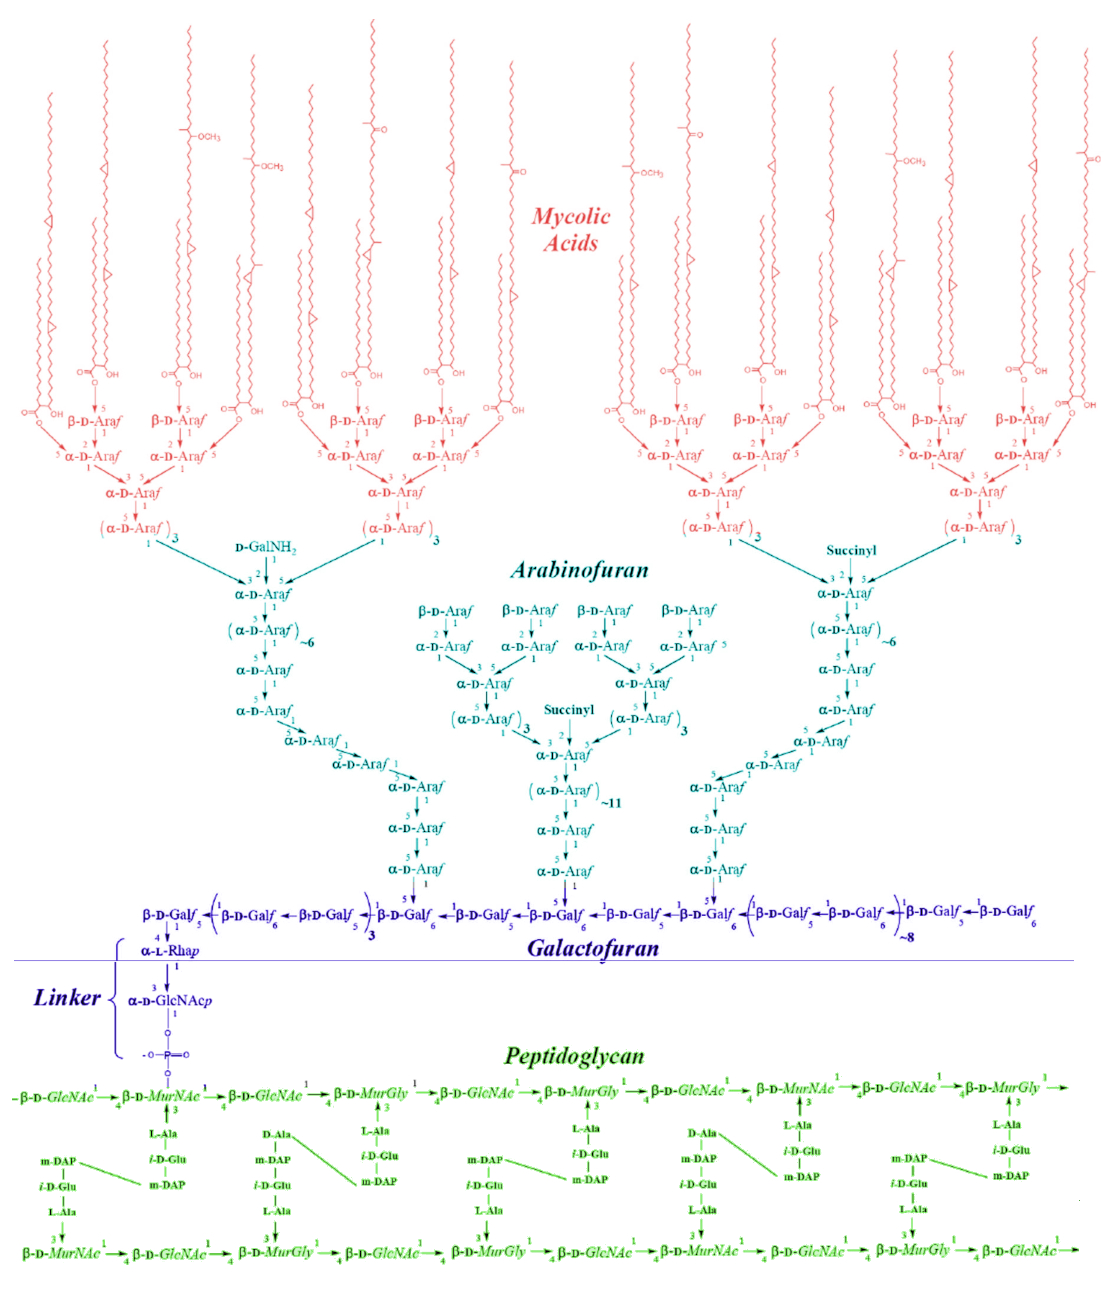
\includegraphics[scale = #1]{fig/iba/mycoliclayer.jpg}}\\[0.3em]
\parbox[t]{0.48\textwidth}{\customlabel{fig:figure1}{\textbf{Figure 1.}} #2}\\[1em]
}
\def\synthesis#1#2{
\customlabel{fig:figure2}
\hfill\mbox{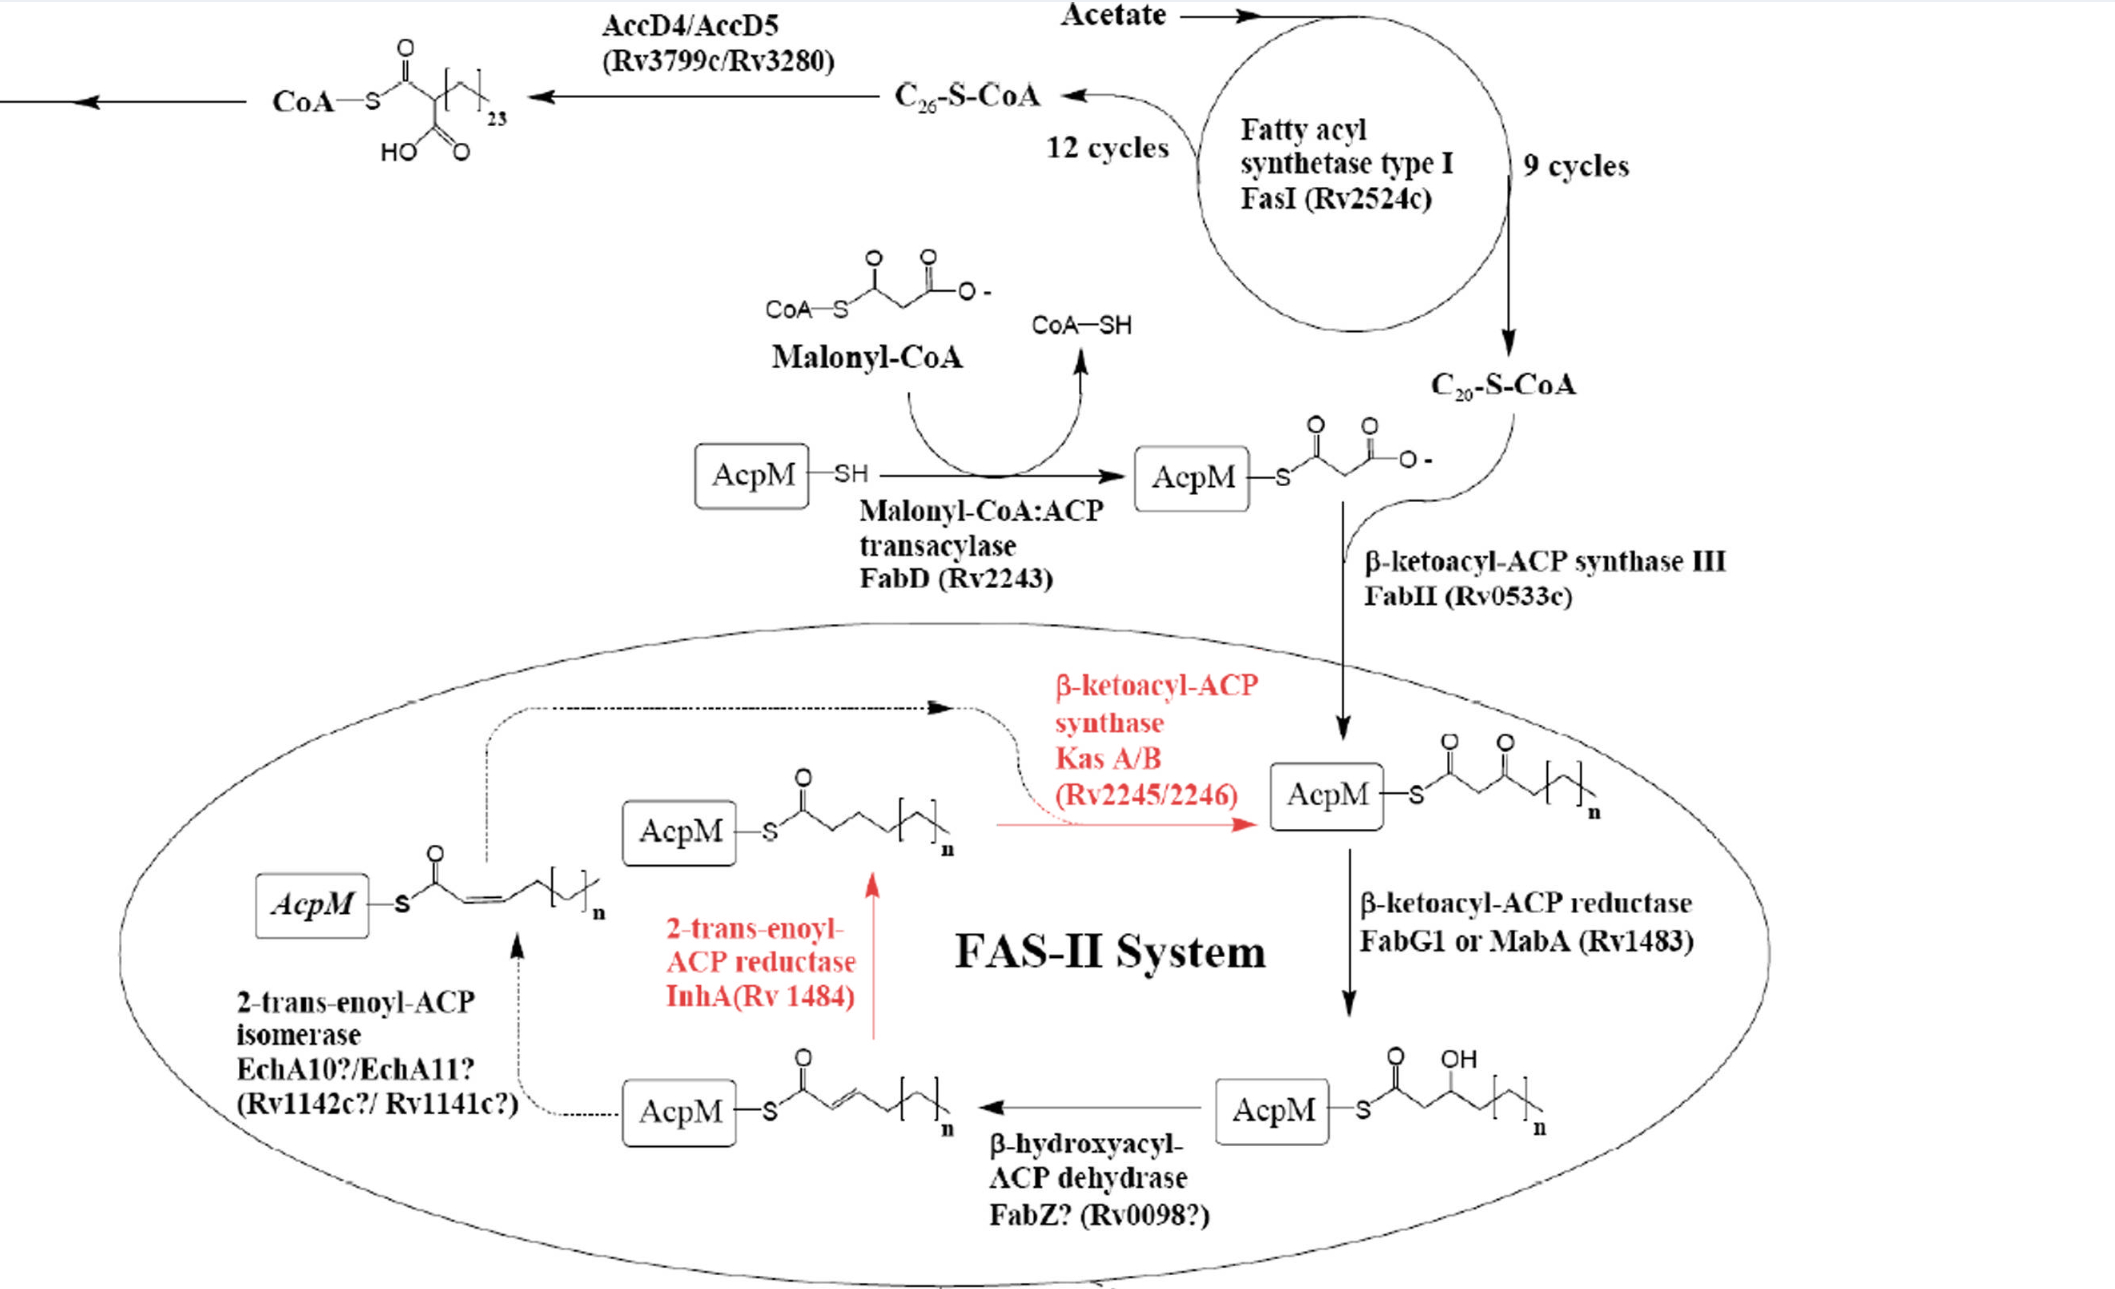
\includegraphics[scale = #1]{fig/iba/synthesis.jpg}}\\[0.3em]
\parbox[t]{\textwidth}{\customlabel{fig:figure2}{\textbf{Figure 2.}} #2}\\[1em]
}
\def\histograms#1#2{
\customlabel{fig:figure3}
\mbox{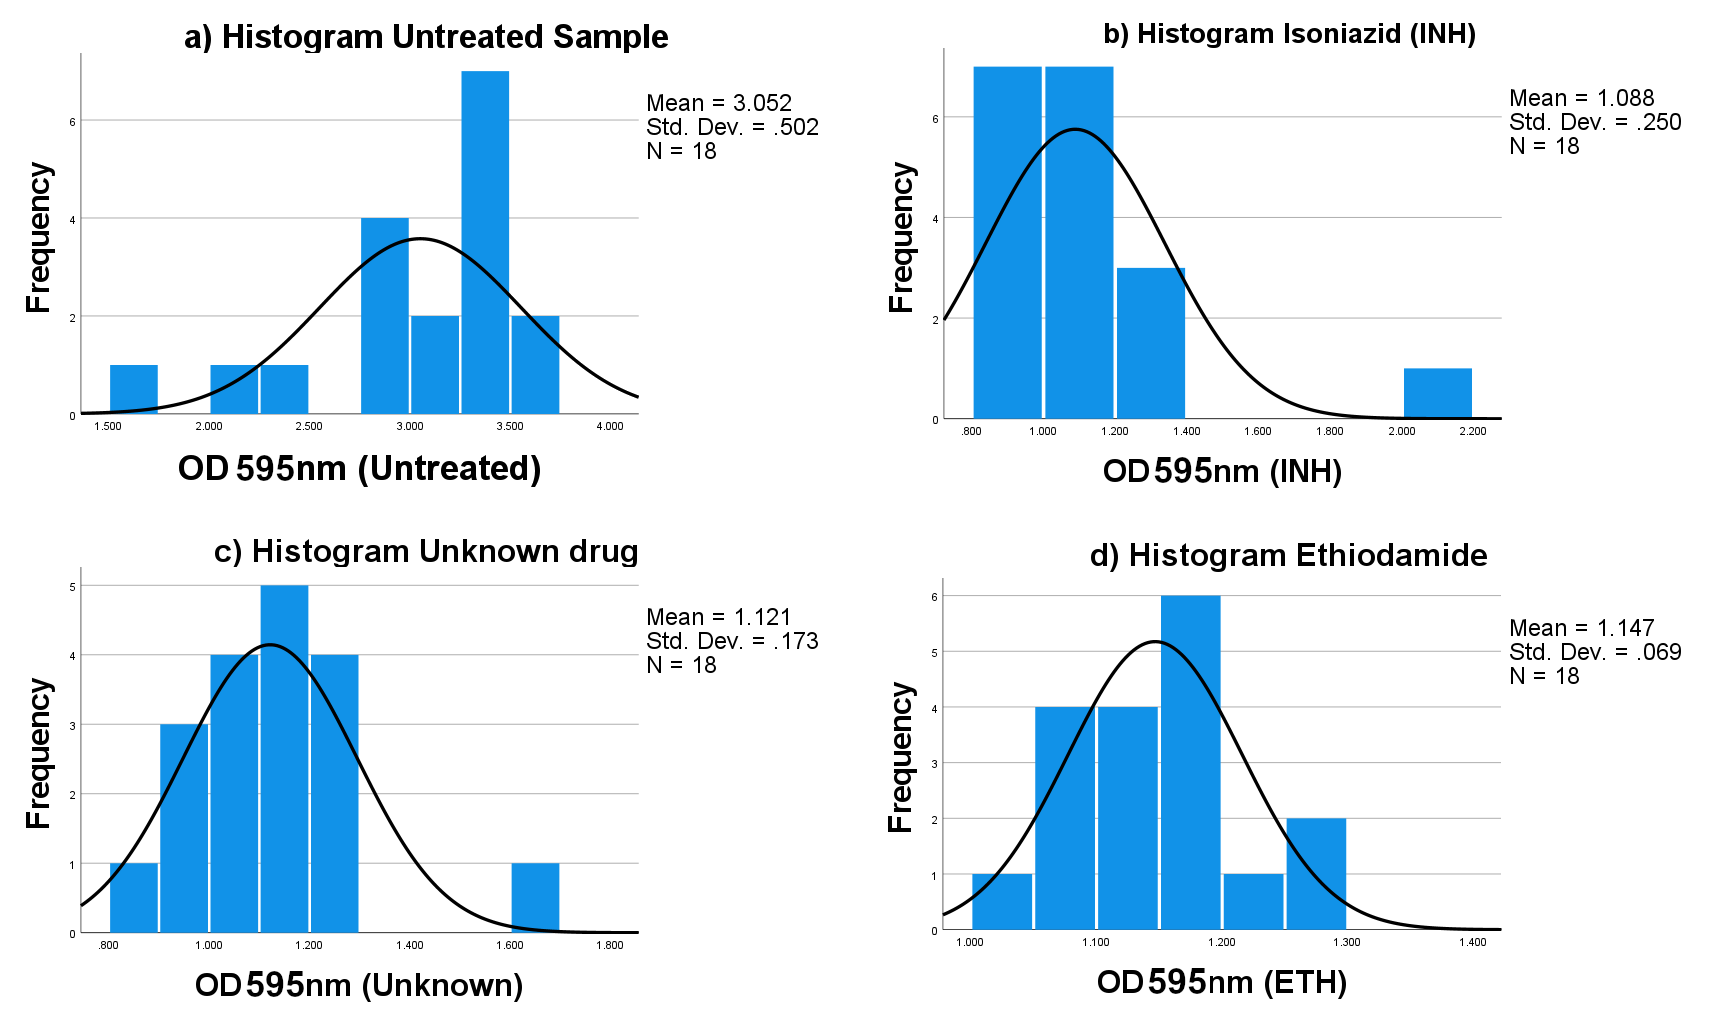
\includegraphics[scale = #1]{fig/iba/histograms.png}}\\[0.3em]
\parbox[t]{\textwidth}{\customlabel{fig:figure3}{\textbf{Figure 3.}} #2}\\[1em]
}
\def\boxplot#1#2{
\customlabel{fig:figure4}
\mbox{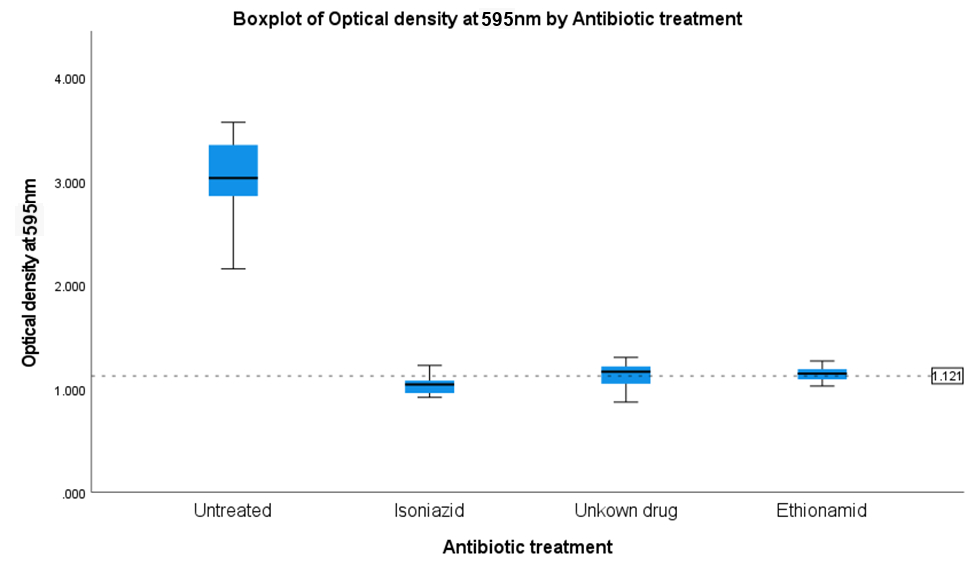
\includegraphics[scale = #1]{fig/iba/boxplot.jpg}}\\[0.3em]
\parbox[t]{\textwidth}{\customlabel{fig:figure4}{\textbf{Figure 4.}} #2}\\[1em]
}
\def\comparison#1#2{
\customlabel{fig:figure5}
\mbox{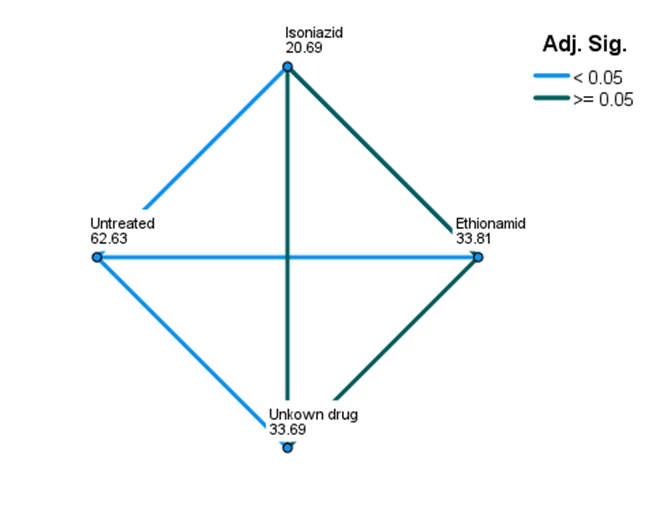
\includegraphics[scale = #1]{fig/iba/comparison.jpg}}\\[0.3em]
\parbox[t]{\textwidth}{\customlabel{fig:figure5}{\textbf{Figure 5.}} #2}\\[1em]
}
\def\UNTREATED#1#2{
\customlabel{fig:figure6}
\mbox{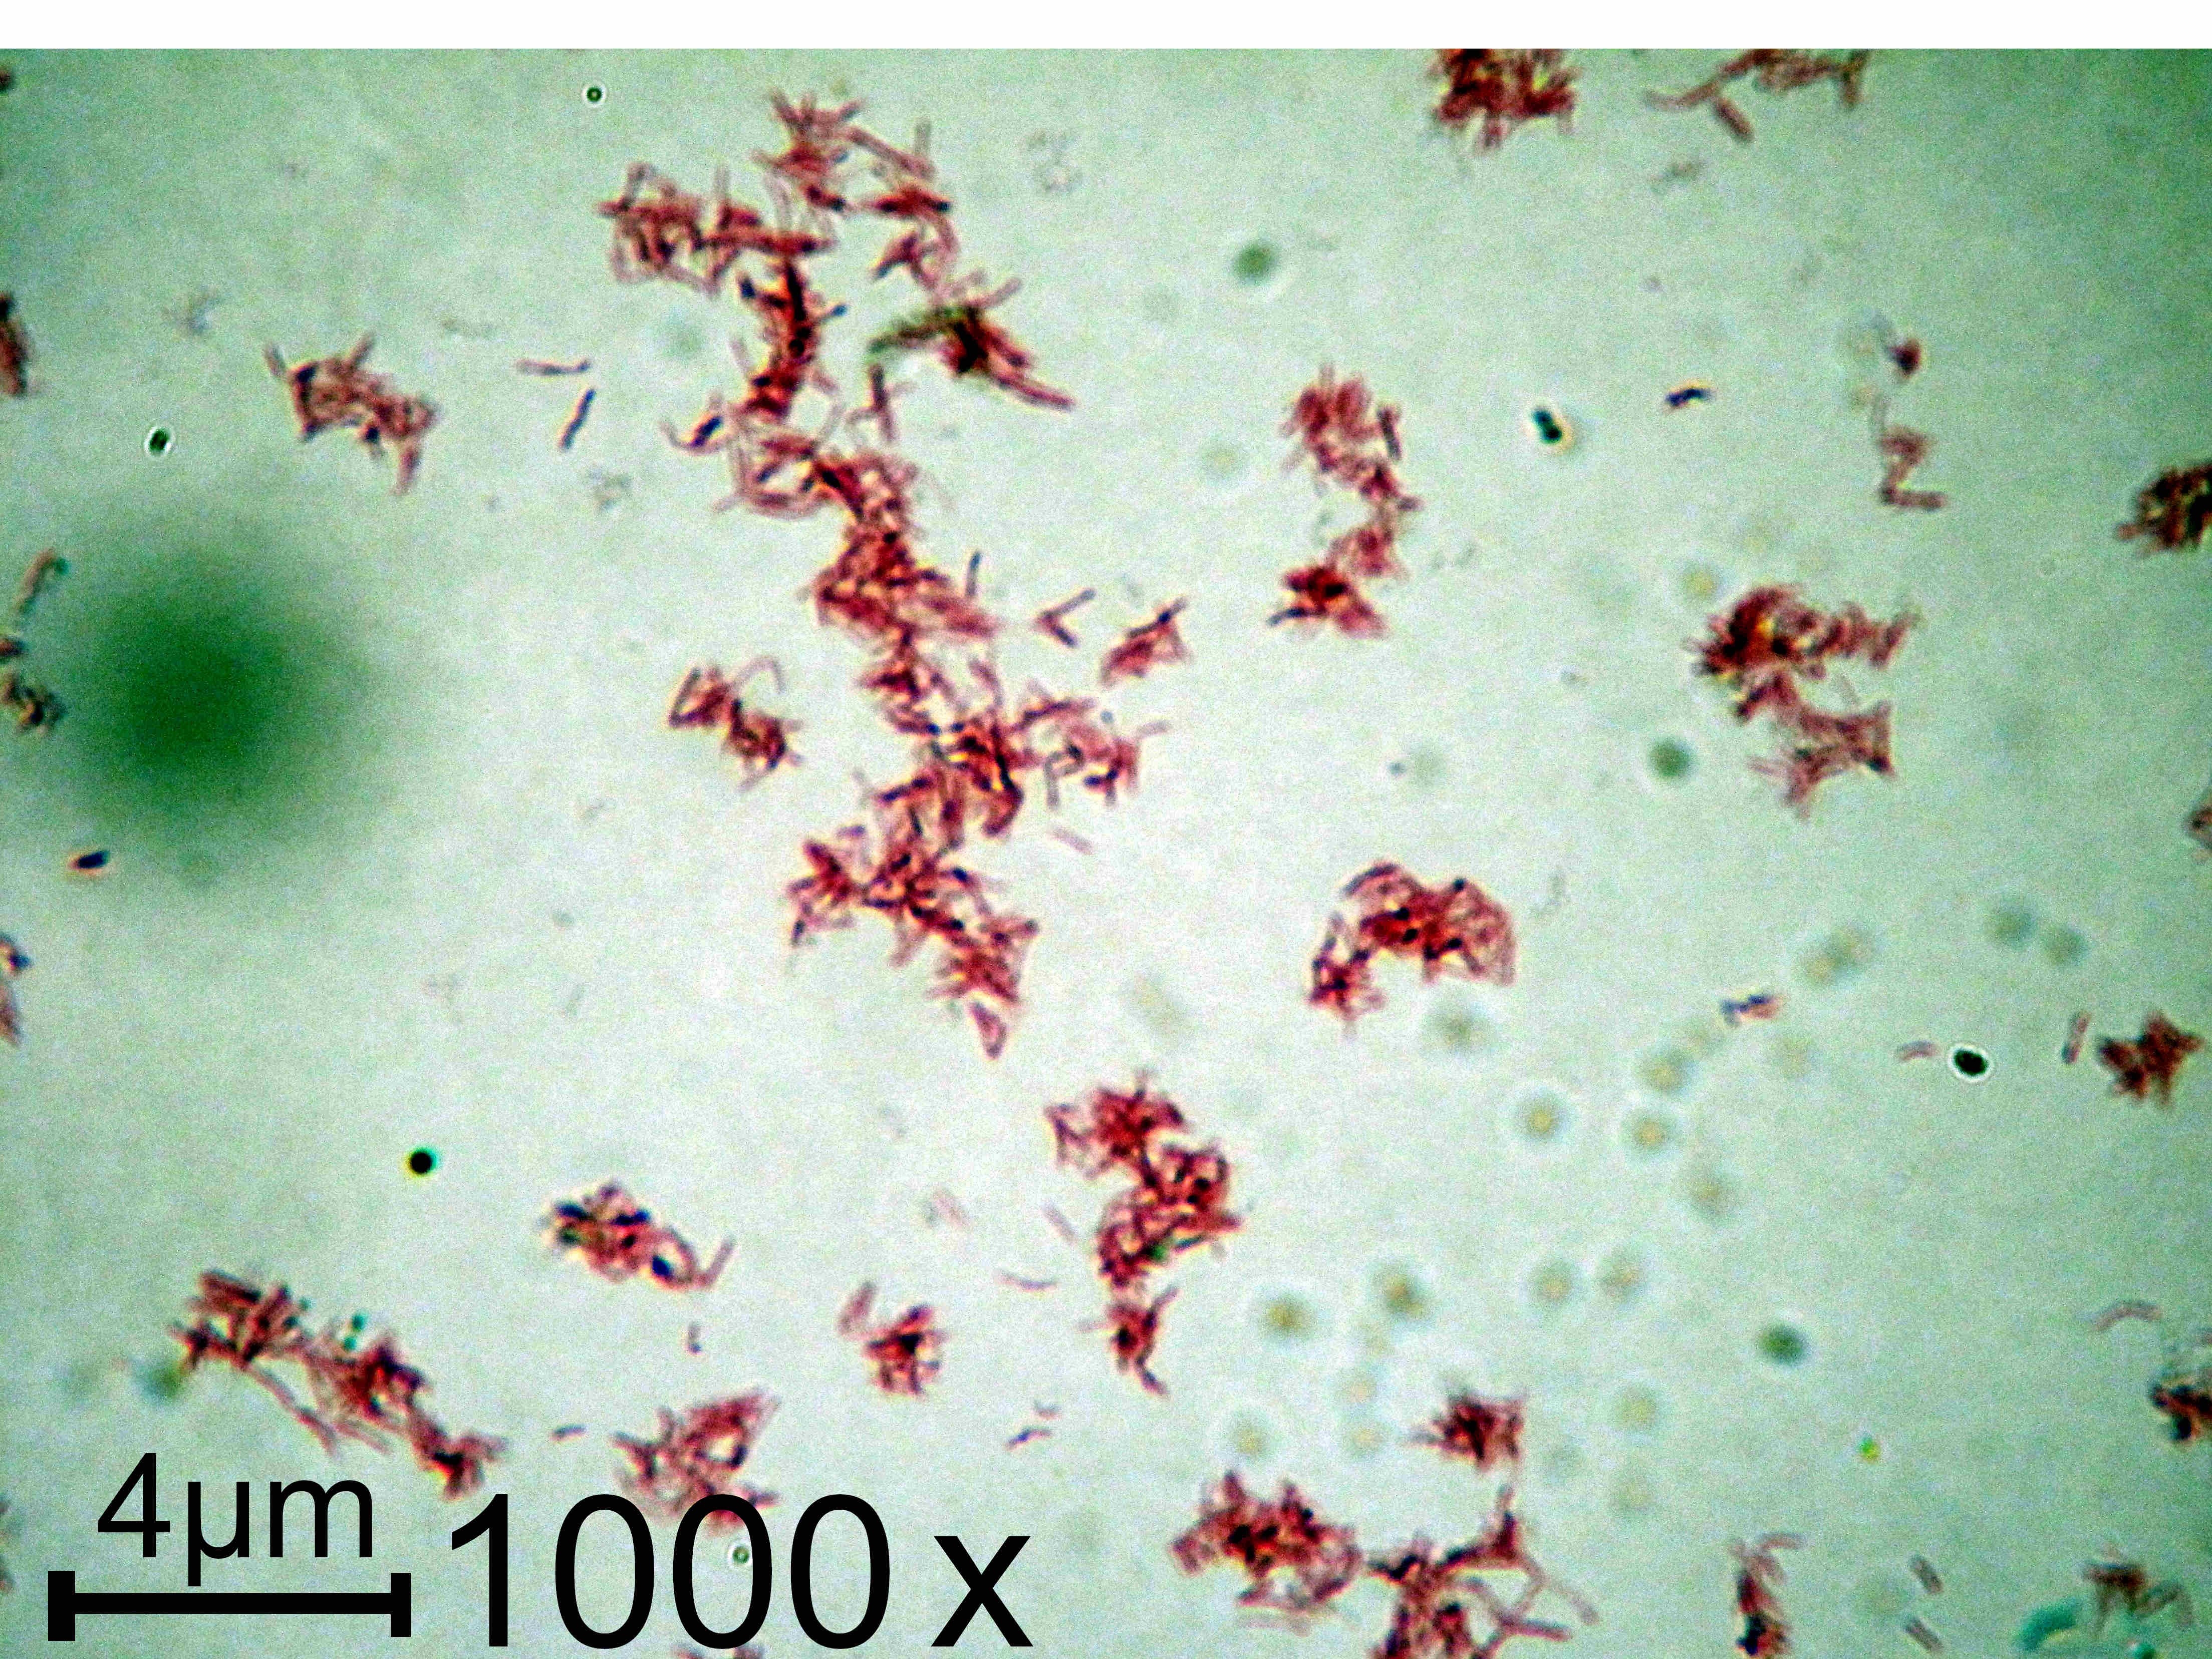
\includegraphics[scale = #1]{fig/iba/Untreated.jpg}}\\[0.3em]
\parbox[t]{\textwidth}{\customlabel{fig:figure6}{\textbf{Figure 6.}} #2}\\[1em]
}

\def\INH#1#2{
\customlabel{fig:figure7}
\mbox{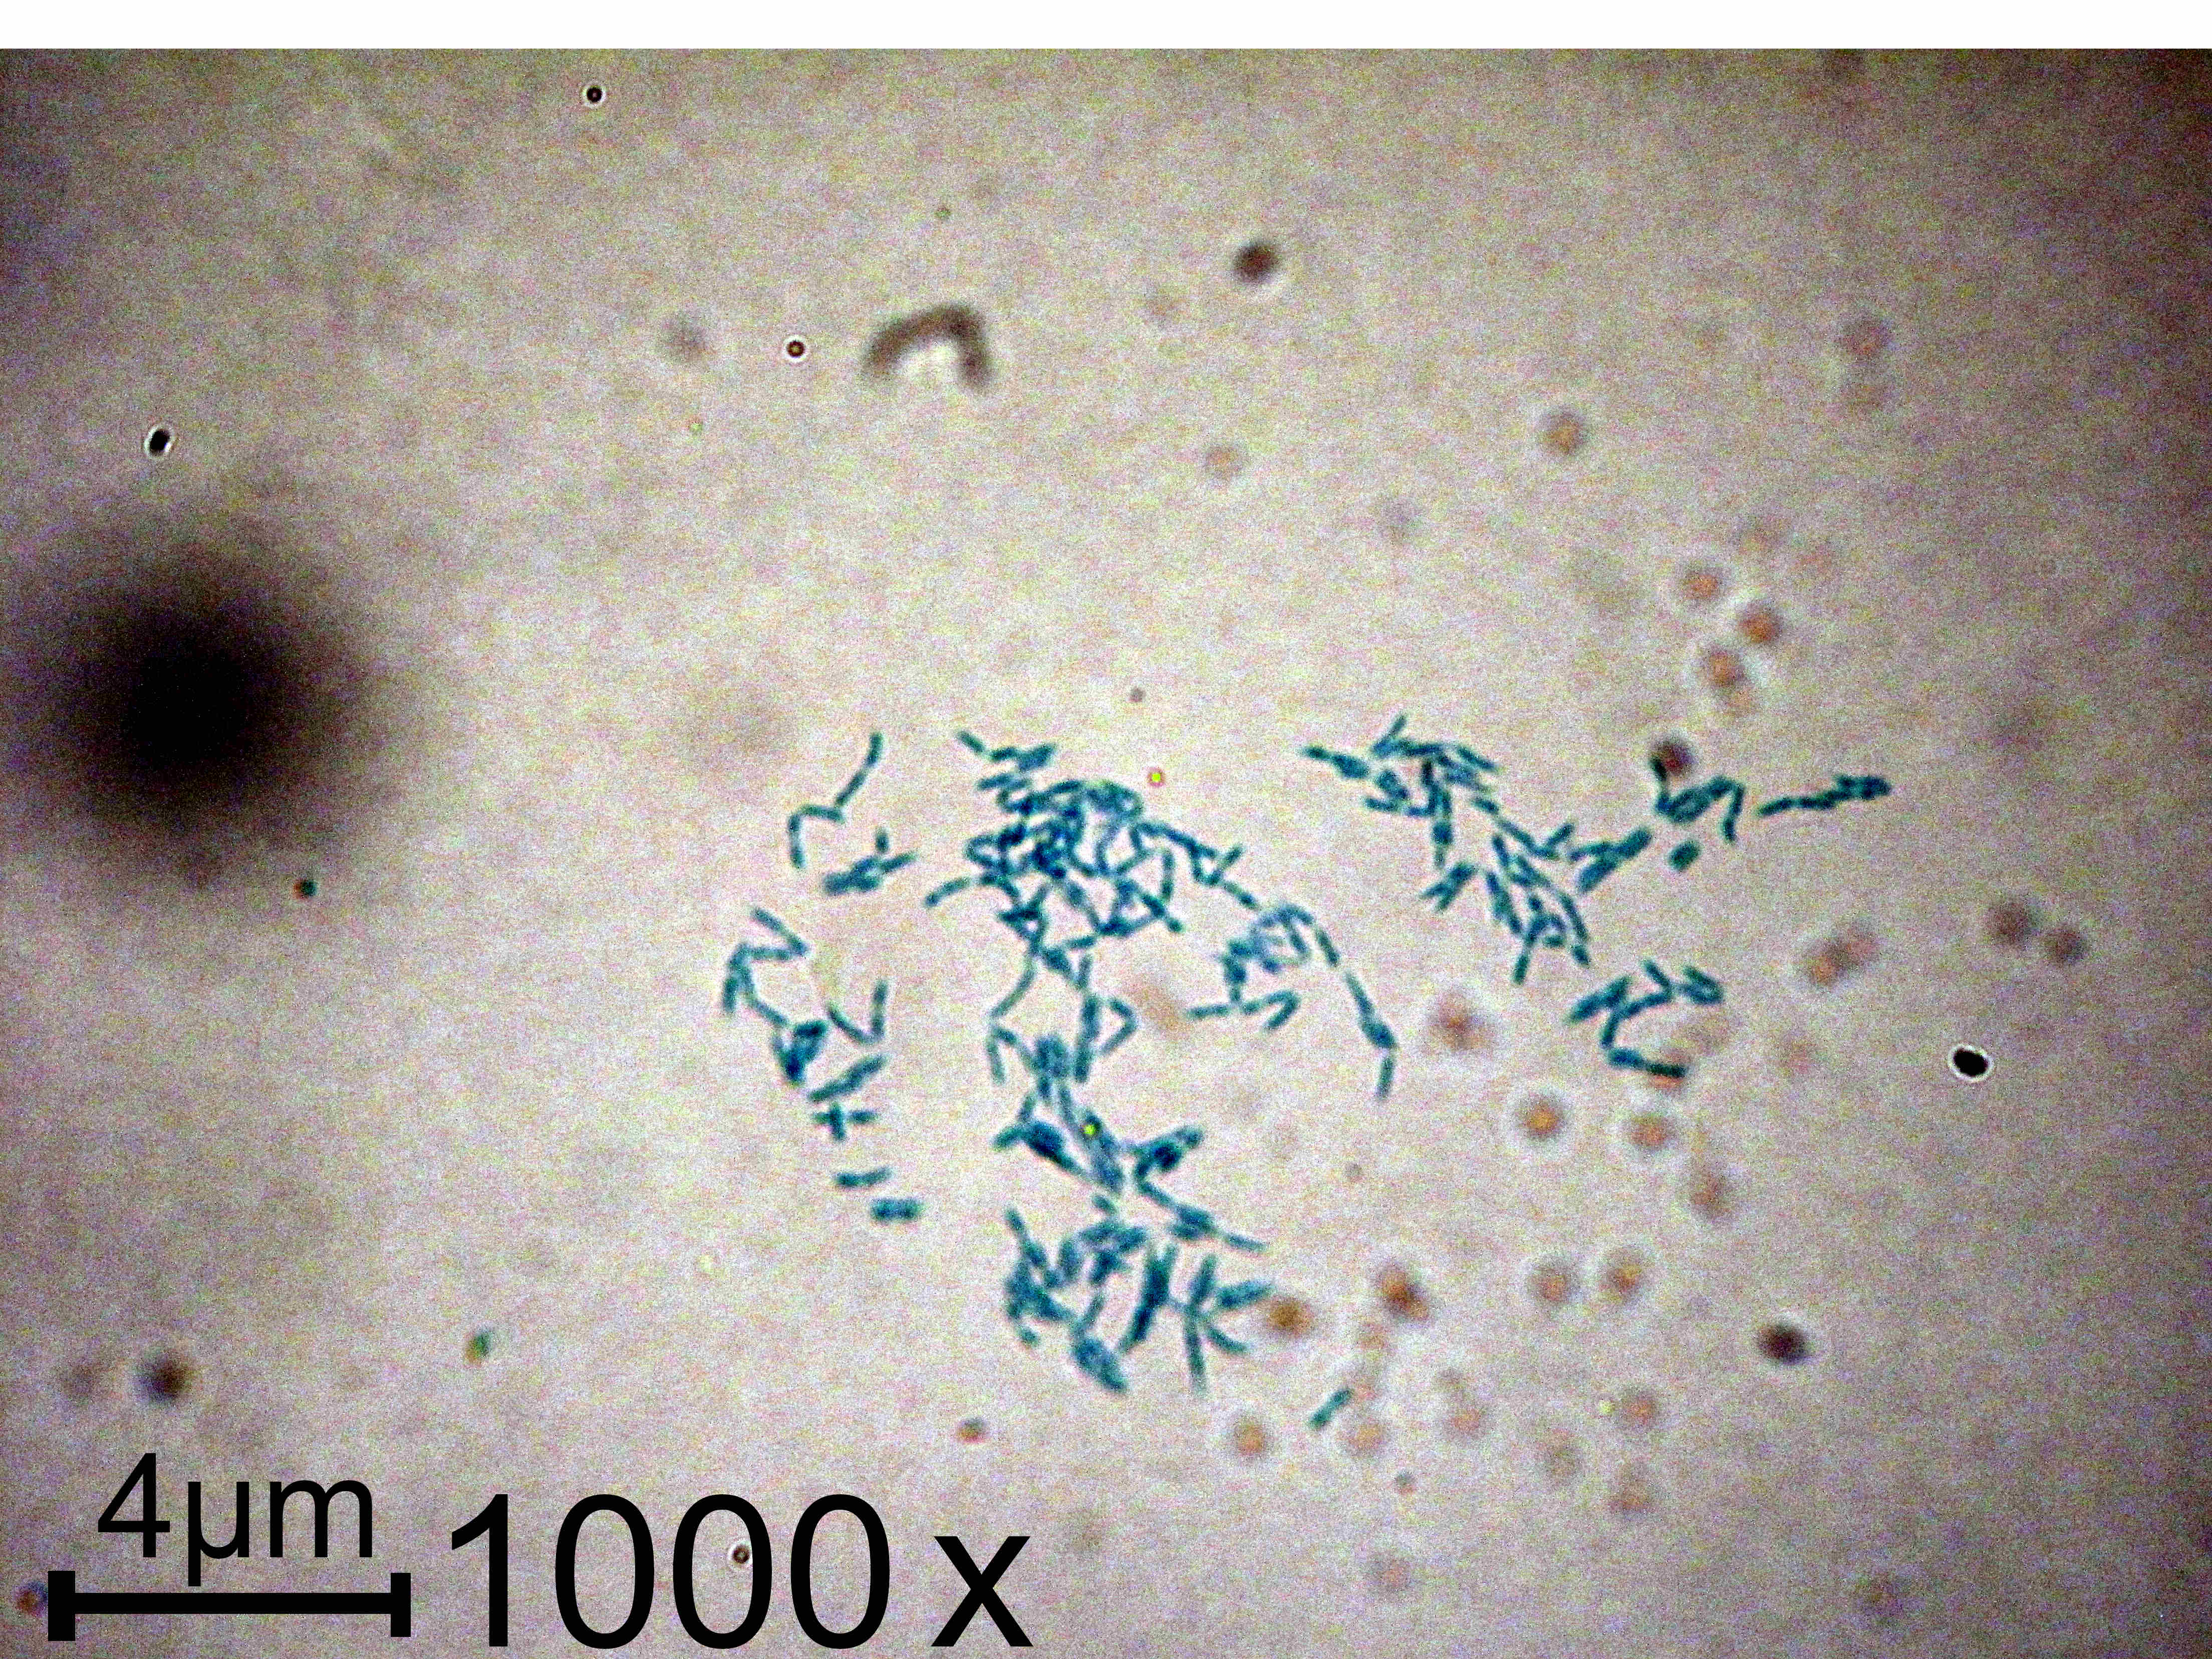
\includegraphics[scale = #1]{fig/iba/INH.jpg}}\\[0.3em]
\parbox[t]{\textwidth}{\customlabel{fig:figure7}{\textbf{Figure 7.}} #2}\\[1em]
}

\def\NCE#1#2{
\customlabel{fig:figure8}
\mbox{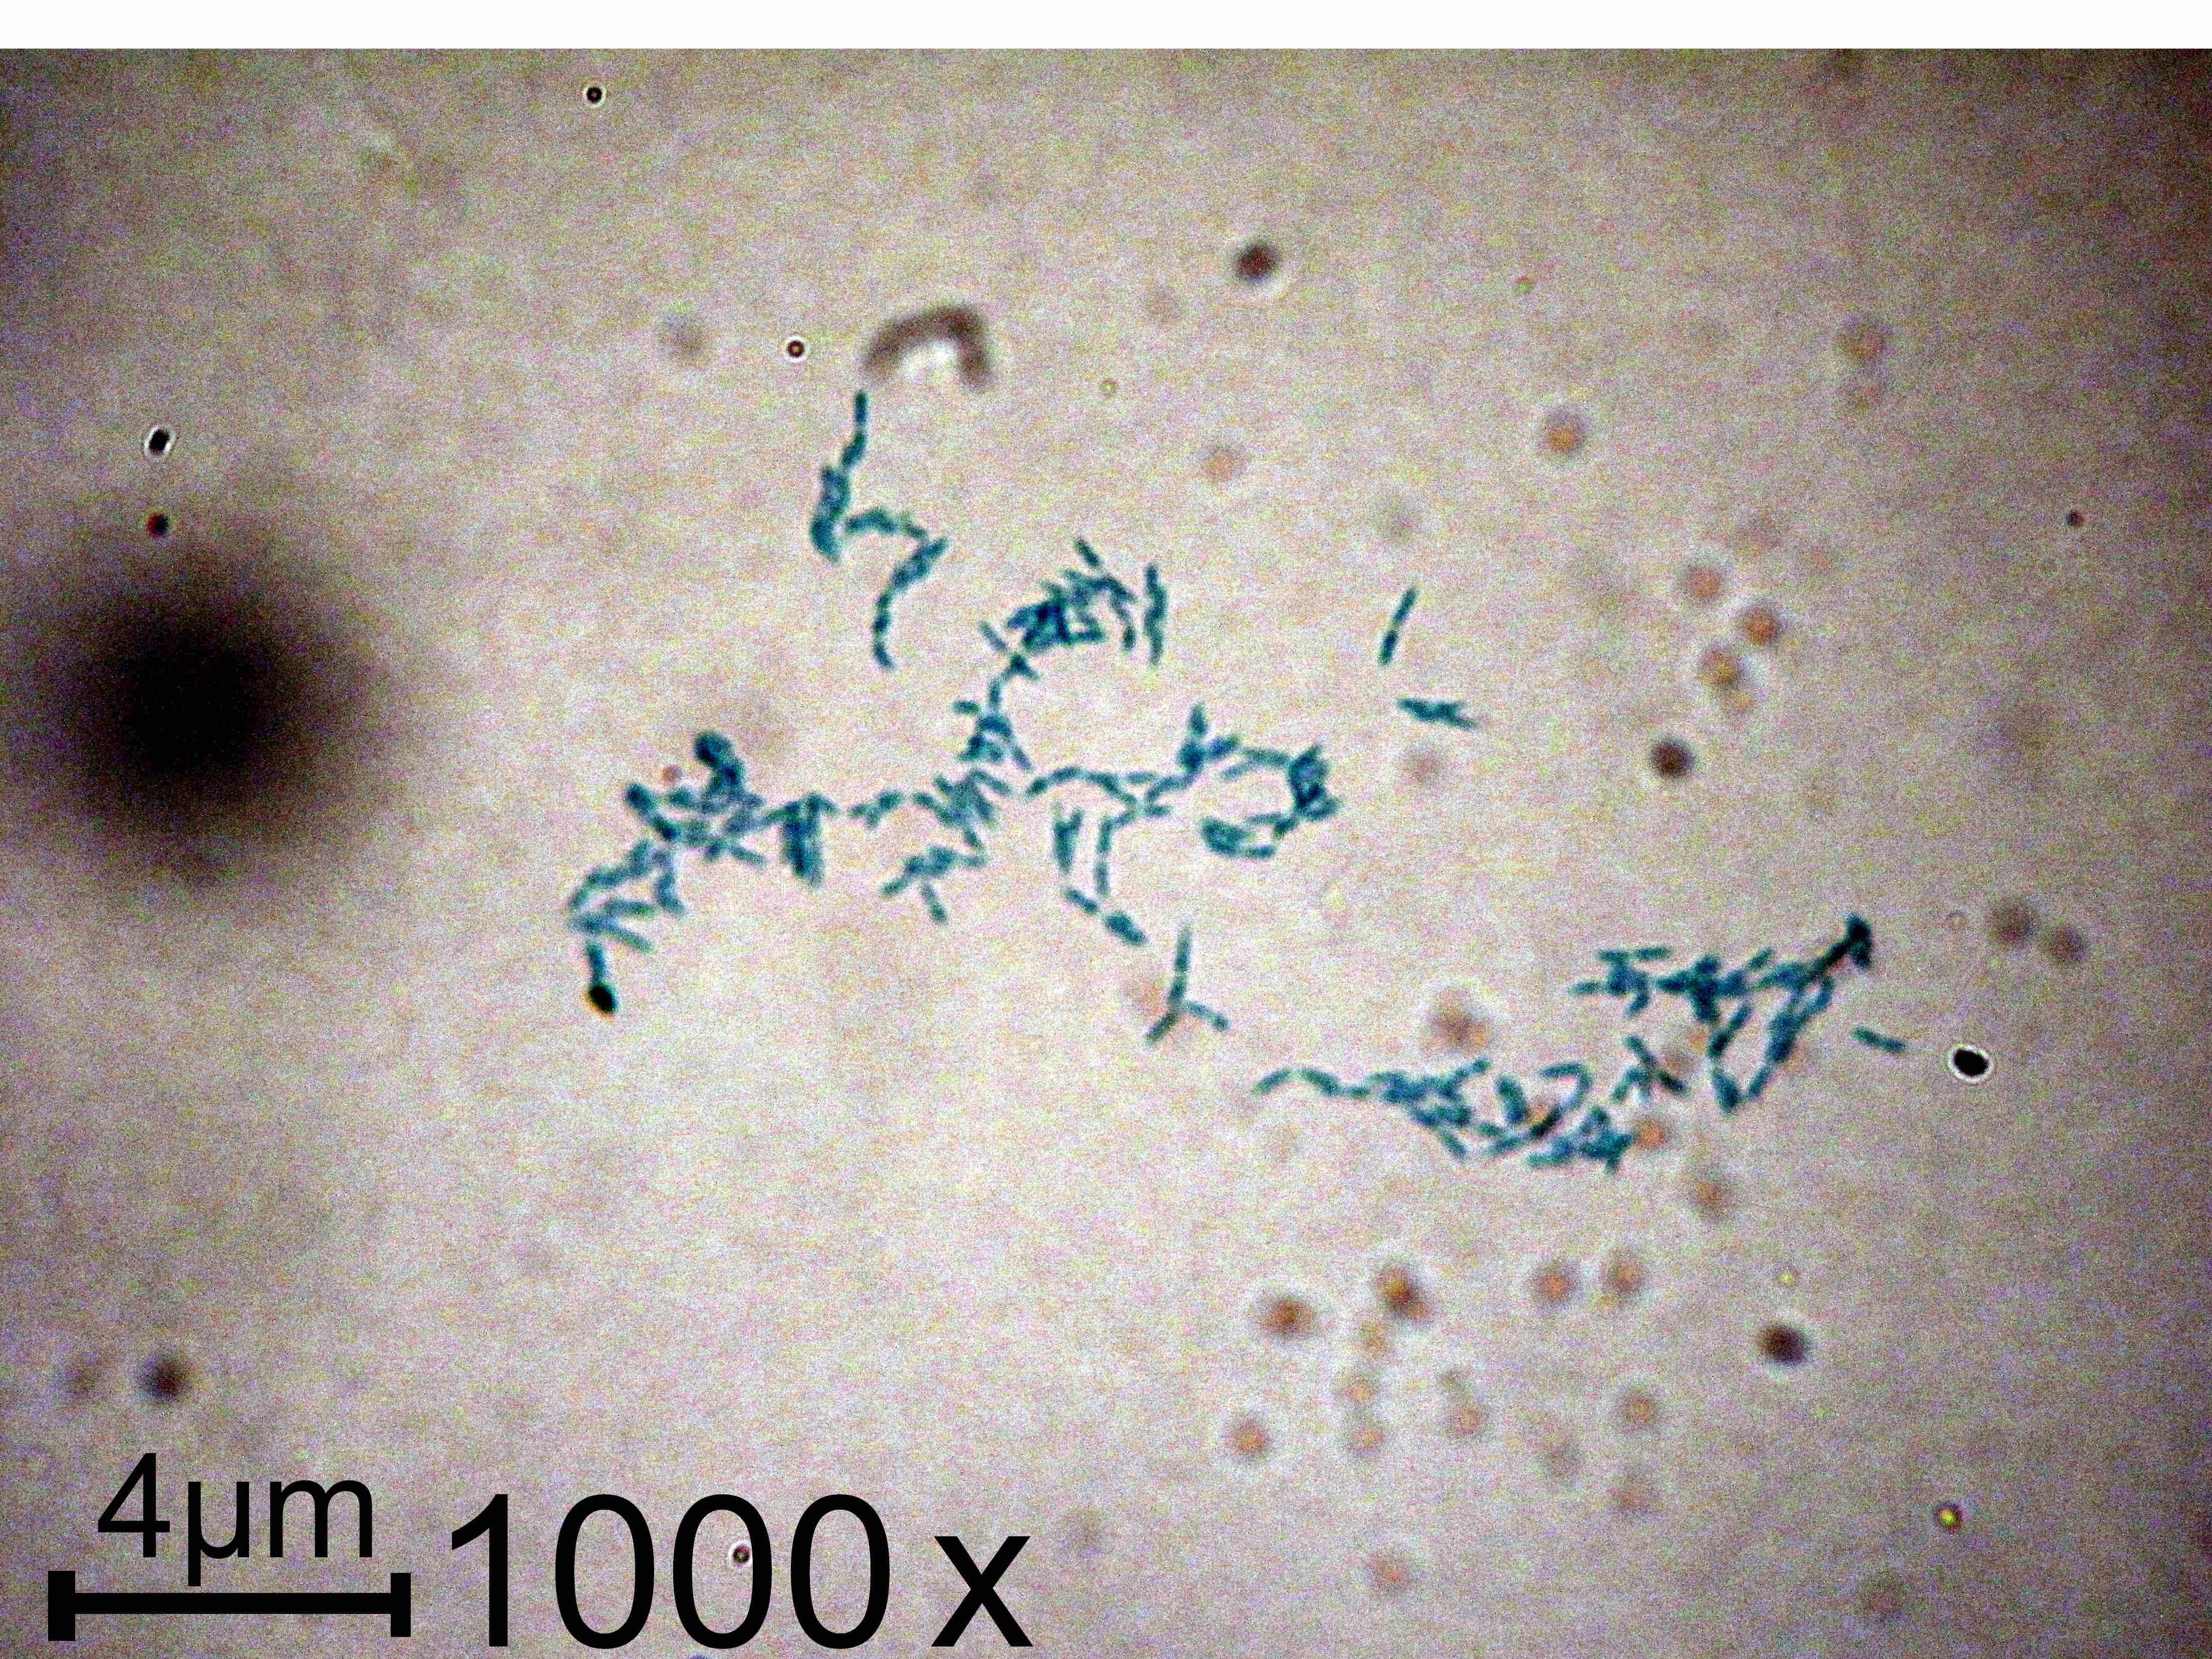
\includegraphics[scale = #1]{fig/iba/X.jpg}}\\[0.3em]
\parbox[t]{\textwidth}{\customlabel{fig:figure8}{\textbf{Figure 8.}} #2}\\[1em]
}

\endinput